\chapter{临时保姆}

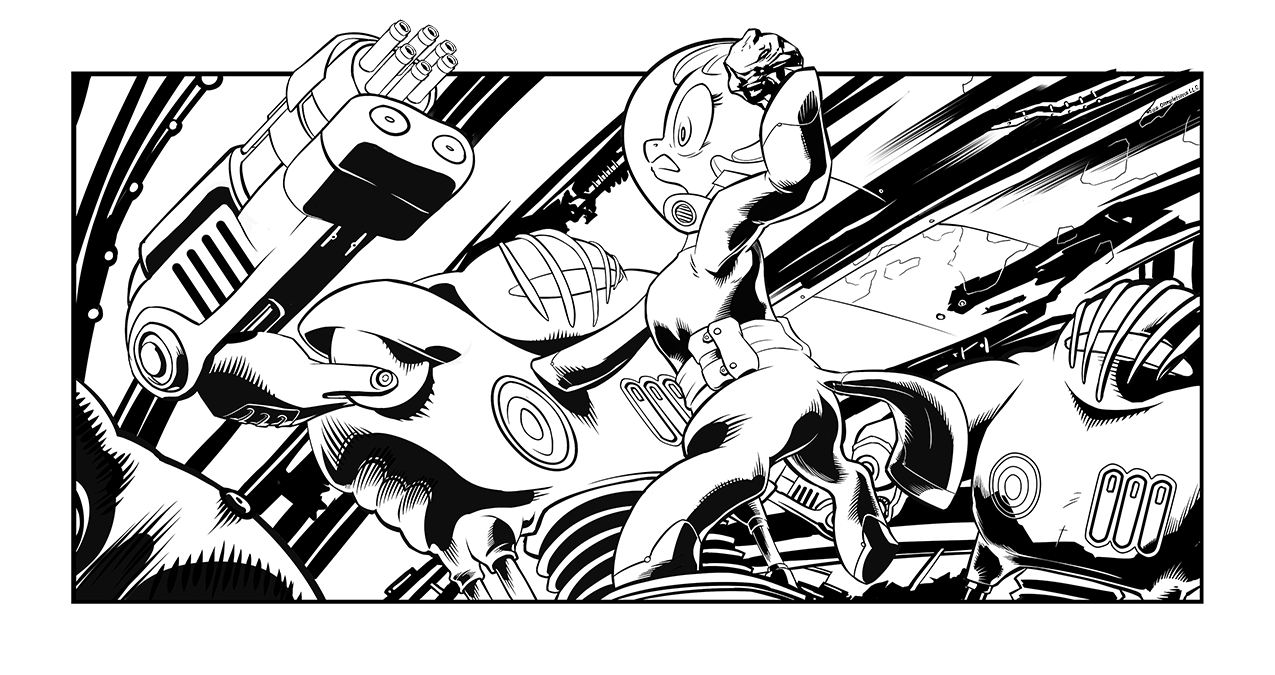
\includegraphics[width=0.9\linewidth]{image07.png}


\begin{intro}
    什么?你说那些可爱的小天使?照顾他们完全没有问题!
\end{intro}

\daytimeplace{6}{9:00 PM}{隧道镇,52号国道北口}{Tunnel Town, Big 52 N Branch}

快乐扳机(Trigger Happy)已经当了半辈子卫兵,她很确定自己见过各种各样想要进隧道镇大门的家伙。不过她现在觉得自己见识还是不够。现在她所有的卫兵同僚都战战兢兢地缩在她背后——只是因为那只穿着滑稽的幼驹现在看起来更不开心了。

「唉,你们这些胆小鬼,算了交给我来吧,你们放松点儿。还有看在我尾鬃的份儿上,别乱开枪。」

独角兽雌驹走出那群卫兵,朝那只被粉色鬼火环绕的黄色小幼驹走去。

「你,就站那儿!别再靠近了,告诉我你到底是谁?」

扳机并没有期待那只幼驹乖乖听话,不过看着她坐下,守卫队长还是松了一口气。

奇怪的孩子挥着一只蹄子向她打招呼:「嗨!我叫快乐帕比!你看到我妈妈了吗?」

扳机皱了皱眉头,「快乐帕比……你就是那个小幽灵帕比?」

「我不是幽灵,我只是个小雌驹!」幼驹嘟起了嘴,她背后还背着一个长长的红色滑板车,看起来不像是武器,虽然的确很大。

「你想说,你就靠一个红板\footnote{红板(Red Racer):飞板璐长大之后开办的玩具公司销售的主打产品,速度非常快的滑板车,虽然对小孩子略有些危险,后来小璐靠卖这个赚的钱和其他CMC一起成立了避难厩科技。}一路从盐块城穿过盐泥沼泽跑到这里?」

帕比咯咯笑起来,「才不是,胖胖独角兽走得超级慢,所以我也得慢慢走。」

「谁谁谁?算了,别提这个了。」扳机叹息着,「我要过去了,你别做……呃……那些鬼鬼怪怪的事情。」

她回头看了一眼,正好和掩体后面露出的三对惊恐的眼睛对上,其中之一还举着一面小白旗晃了晃。她真心向女神祷告,祈求能有几个更靠谱的队友。然后她走向帕比。

「嗨!你好漂亮!漂漂小马姐姐!你叫什么名字?」幼驹露出她最友善的笑容。

\thpr{她只是……只是……只是一个有对发光双眸的幼驹而已,估计只是受了点辐射影响。}「没搞错吧,你就是新闻说的那个快乐帕比?那个来自盐块城和嘉年华的幽灵?」卫兵笑了起来,「拜托,别扯了!」

帕比也跟着笑了起来,「哈哈哈!很有趣对吧!呃……不过哪里有趣了?」

幼驹的问题让卫兵队长笑得更响了,「快乐扳机,但你叫我扳机就好。」

帕比皱了皱眉头,「啊,我能叫您乐乐么?」

「当然,对了,我还有个东西……」扳机拿出一片黄色的塑料卡递给帕比,「这是你的通行证,中午有个叫赫瑞塔的狮鹫来到这里,她一直等你到傍晚,但是你还没来,所以她先走了,不过她走的时候还帮你交了通行费,她说你最迟明天就会来。」

「呃,赫瑞在这里?她还好么?」

「我想……她很好,不过她不太爱说话,不过我也没碰到过爱说话的狮鹫。」扳机扭头往回走。「进来吧,在外面可不利于健康,附近可有不少血翼\footnote{血翼(Bloodwing):吸血果蝠受辐射影响以后,真的吸血了}。」

「血翼是什么啊?」帕比跟在扳机背后问。

「如果你问我的话,他们就是麻烦!是长翅膀的大号水蛭!」雌驹笑着伸蹄子招呼帕比走进去。里面是一间用沙包和生锈的铁板围成的简易窝棚,两挺加特林机枪在窗口前指着桥头,而墙角堆着一大堆弹药箱——还有三只全身紧绷的小马一脸尴尬地打着招呼。

「伙计们,别这样。这是快乐帕比,嘉年华的小英雄,她和我们可是一伙儿的,所以别害怕好吗?」卫队长举起蹄子掩嘴窃笑,「我还真想看看孤狼亲眼看到他所说的『英雄』是什么样子会有什么反应。哦,这几位是绿梨,坏枪和小豆子。」

「嗨!我叫快乐帕比!」幼驹蹦跶到仨小马面前。看着她的新朋友们一脸紧张的表情,于是她又接着说:「我正在找我妈妈!她或许会在山里面!」

三个守卫之一低声嘟囔着:「这下麻烦可大了……」

\horizonline

\daytimeplace{6}{9:45 PM}{隧道镇,52号国道北口}{Tunnel Town, Big 52 N Branch}

「哇塞!好大哦!」帕比看着隧道入口,一直仰头到一屁股坐在了地上。这个隧道大到可以同时让天空马车和普通马车一起出入,而且有两排车道!隧道的混凝土墙壁在深入山脉20米之后,被一道生锈的巨大铁门硬生生地截断了,那面铁门上是一个白色的天角兽标志,看起来那标志简直比女神更雄壮威武。标志下面是一行字:旭日公司——走可持续发展道路,而字下面,又是一个平常门上都会有的大大危险警告标志。

「看到了吧。」扳机敲了敲那个金属大门,「它封死了,我很抱歉,小家伙,但是这估计就是你旅程的终点了。」

「但是……妈咪在里面!你看那个箭头!它指着大门呢!我得进山里面去!请打开它,拜托!」帕比闪着水汪汪的大眼睛。「超超拜托,漂漂的乐乐姐姐!」

卫兵队长后退了一步,「哎呦,这眼睛绝对该列为违禁武器……不过,我很抱歉帕比,就连我们自己也没办法进去。为了打开它,我们都不知道试了多少次了,不信你看吧,我们现在还是零分。」

「但是我真的,真的,真的真的真的要进去!妈妈在里面等我!」小雌驹满地打滚。

坏枪摩挲着自己的胡茬子,低声地自言自语:「我想那个TNT曾经说过可以从通风管进去?」

扳机瞪了他一眼,「闭嘴!」然后转头满脸堆笑的看着帕比。

「懂了么,没办法进去!」她想板起脸,但是小雌驹早已经不吃那套。

「呃,洞风道?那是啥?拜托,告诉我!我为你做什么都行!哦哦哦,我拿这个跟你换!」帕比忽然掏出一个从军事基地拿出来的坦克炮弹头,这一个上面是黑带,「你看,这个闪闪发光的东西超级厉害!您让我进去我就给你这个!成交么?」

「帕比……这危险了!我不想让幼驹去送死,抱歉。」

幼驹后退一步,看起来她就快要哭出来了。「我才不怕!这不公平!如果你们妈妈被关在里面你们肯定早就打开这破门了!而且……而且……」小雌驹尥蹶子踢着门。「我不能在这里放弃,她在里面!她一定在里面!」

坏枪趴在扳机身边耳语着:「为什么不让她进去,她已经救了俩城市了……我可不觉得她只是个一般孩子。」

独角兽卫兵叹了口气回答:「我们现在根本不知道隧道里面有什么,你好好想想大门关上的那天,我可以清楚地听见困在里面的小马敲门呼救的声音,还有枪声和惊恐的尖叫。」扳机用蹄子敲着坏枪的前额,「你好好看她,就算她也许是个不一般的小家伙,不过她也只是个孩子!我绝对不会送个孩子去踩雷区!」

公马卫兵注视着他上司的眼睛,「你觉得她会就这么放弃?如果她真的是那个幽灵,那我觉得我们也没什么办法阻止她。」

快乐扳机以蹄扶额摇着头,「你还真信那些床边故事?拜托,醒醒吧,她就只是个穿着全套防辐射服还稍微受了点儿辐射影响的小孩子而已!」

这个时候帕比依然站在大门前垂头丧气,「我不是小孩子,我长大了……我还能放飞气球!」她愤愤地朝扳机皱着眉头。帕比脑袋里忽然冒出一个新点子,小雌驹抬起了头,「喂,声音先生,他们说的那通风洞是啥?」

「{\mt 通风道:排风系统,用于将新鲜空气吹入密闭空间的设备,大型隧道使用的通风道通常可以允许小马爬进去以便进行维修——知识小点滴!}」

「哦,酱紫啊……怎么进去,维……维什么那个东西?」小幼驹活用她刚刚学到的知识问道。

「{\mt 肯定,读取地图,旭日公司,2号隧道,分析技术蓝图,警告,部分蓝图属于军事机密无法展示。读取A01,A02,A03部分,读取维修管道蓝图,分析中,检查线路,维护仓A01-104设为新目标点。}」

粉色的箭头从罗盘上消失,然后指向新的方向。

帕比的小嘴上露出一个得意的笑容:这就是所谓的智取!

\horizonline

\daytimeplace{6}{10:15 PM}{隧道镇,52号国道北口}{Tunnel Town, Big 52 N Branch}

「我可得说,从来没有见过哪只小马能装在密封防辐射服里忍三天以上的!你这所谓的『小鬼』可一点都不普通!」

坏枪指着帕比应该在的方向,但是那里现在却只是空地,然后他们才反应过来,领悟到了一个事实:他们居然让那么大一个黄澄澄的小幼驹从他们眼皮下溜走了。「我勒个去!」

快乐扳机惊得跳了起来,着急地看着四周问:「她一分钟前还在这里!你们怎么就没把她看好?」

「好吧,现在我的工作又加上了照顾一个黄色小马灯泡了!你还想干啥?」坏枪耸了耸肩。「你看,就像我刚刚说的,52号国道的幽灵是不可阻挡的。」

「别叨叨了,她才不是幽灵!」快乐扳机挥着蹄子表示不认同,但是她的伙伴还在继续说。

「拜托,乐乐,你就听我一句好不好,别惹闲事了,这地方已经一天不如一天了……我们小时候光着屁股在52号国道乱跑的时候,外面哪儿有那么多的奴隶贩子和废土强盗?每个小镇都有足够的力量保护每个镇民……」然后公马叹了口气,「难道你不怀念那些日子吗?」

雌驹有些哀伤地低下头,「没错,那个时候日子很开心,隧道还常通,而且太阳城还是个文明的大城市……但是现在52号国道只剩下一大堆法外之徒。」

「没错,所以我想说,大家总说『万物皆有灵』,对吧?」坏枪觉得自己的词汇量不太好解释自己的想法,「就像一个大城市,很多小马住在里面的大城市,所有家庭都在努力让城市变得更好,好像整个城市就是一个活着的整体一样。」

「没错,那就叫做社会群落……你想说啥?」扳机不解地看着公马,「你最好能赶紧说结论,因为现在我们刚走丢一孩子。」

「所以,52号国道也是类似的东西吧!我是说,赤兔,白苹果,清砂工还有其他氏族……或许他们都是独立的,但是我们都在这条从首都到翡翠海岸的大道上,所以我们都是52号国道的一部分。」

坏枪举起一个蹄子从北向南比划着。「盐块城属于白苹果,但是52号国道属于生活在这里的每一个小马!」

「这演讲真是动听啊,但是我不明白这和找帕比有什么关系。」

「我马上就讲完了,我们都有那种感觉,现在52号国道正在生病,和小马国的其它地方一样陷入了噩梦,但是忽然……乒!这个幽灵就冒出来了,而且开始解决那些烦恼我们几十年的问题。」

「赤兔氏族都快灭绝了,因为嘉年华每年杀死的幼驹不止一只,它正在杀死未来和希望。我早就听说那里的雌驹都不想怀孕,因为他们害怕失去孩子,而那些尸鬼呢?你知道每年有多少车队大老远绕道去荒芜之地然后才能到岩块城?」

「好吧,你说得没错,但是我可不觉得那孩子能……」坏枪打断了扳机。

「我觉得她能行!」坏枪坚定地说。「想想今天那个狮鹫,你看她的双眼了么?她眼中那种……光明……就好像有什么事情烦恼了她一生,但是现在事情好转了,她眼中有希望,而且满怀感恩之情。想想吧,乐乐,在这个破地方还有多少值得感谢的小马?或许几天之前,大家之间还有最起码的信任,但是现在呢?如果没有通行证,你啥都不是。」坏枪顿了顿,但是扳机没有说话只是听着他。

「现在她应当走进那隧道里,或许她只是个幸运小鬼,或者是个死掉的小鬼,但是,我想要相信它不仅仅是那样,虽然她不是避难厩英雄\footnote{避难厩英雄(Stable Dweller):\emph{FoE} 主角 LittlePip 在废土上的称号},也不是废土卫士\footnote{废土卫士(Security):\emph{FoE: PH}(\emph{Fallout: Equestria - Project Horizons})(《辐射小马国:地平线计划》)主角 BlackJack 在废土上的称号},但她是我们的希望,就像是……老朋友52号国道正在想要自己解决一切麻烦一样。」

快乐扳机叹了口气:「你是个无可救药的傻蛋梦想家,如果你遇上什么困难,你不能坐在那里干等着有个英雄出现,你应该去面对它,然后从中学到什么。」雌驹望着阴云密布的夜空,「不过有一点我同意你,这孩子根本不知道什么叫放弃。我知道她去了哪里,如果我就这样让她去给自己惹麻烦,露娜会诅咒我一辈子。」

\horizonline

\daytimeplace{6}{10:15 PM}{旭日公司隧道,隧道镇}{Solaris Tunnel, Tunnel Town}

金属刮擦声回响在通风管内,整个地方都漆黑一片,除了帕比双目的光芒和头盔闪烁的HUD。不过对于小雌驹来说,足够她看清眼前的路,只要跟着箭头走她就不会迷路。

「等我找到妈妈,我要给她一个大大的拥抱,然后她也会亲亲我,然后我们就永远在一起了!」幼驹一边预演着她整个计划最重要的部分一边说:「这一次她绝对不会走了吧,对吧,声音先生?」

「{\mt 否定,计算表明,您的雌性血亲不在的概率为……99.9\%}」

「别说那种事好吗!要保持乐观积极的态度!」帕比停下来看看四周,她可以发誓她听到了什么,「你听到了吗?好像有小马在喊叫?」雌驹深吸一口气,「我在这里!你在哪儿?」

帕比的声音在黑暗的通风管里面回荡着,似乎远处有个声音回答,但是帕比听不清。

「那声音从哪里来的?」

「{\mt 分析中,该地点白噪音太高,无法确定音源。}」

「那好,我们继续走!」帕比发现她脚下有个通风口,在下面就好像是像要吞噬一切的黑色虚空。

「呃……为什么箭头指向下?」

「{\mt 读取介绍中。你必须穿过维护仓A01-001的通风口以达到主隧道地面。}」

\horizonline

\daytimeplace{6}{10:15 PM}{隧道镇,52号国道北口}{Tunnel Town, Big 52 N Branch}

「我才懒得管你的破理论,快给我把头灯拿来,然后看看清单上缺什么。」快乐扳机穿着一身快磨破的维护服,还带着各种各样的工具。

坏枪叹了口气,想要表现得更烦恼而不是担心。「随你便,乐乐,但是……拜托一定要回来。」

扳机嗤之以鼻,转过头去:「清单!」

公马又叹了口气,

「绳子。」

「带了。」

「电池。」

「带了。」

「罐头。」

「带了。」

「霰弹枪。」

「带了。」

「子弹。」

「带了。」

「常识。」

「带……喂喂,别玩儿了好么?」

这回坏枪先发火了,「你这是在自杀!你虽然枪法很准,动作也很灵活,但是你只是一只小马!你会送命的!我不想失去你?」

雌驹回过头来,「失去我?你是啥意思?」

「我想说……我爱你,快乐扳机!从我们还是小孩子的时候就开始了!你觉得为什么我要进卫兵队而不是继承老爸的酒馆?别去,或者至少让我跟你一起去!」

扳机皱起了眉头,「你是想说……你对我一见钟情了……大概……20年然后一个字没提?就算黑帽子和我……」扳机摇了摇头,「你是在玩我吧,是不是又在拿我开心?」

坏枪低下了头,「我真希望是,但是你有时候总是很无情,我又有点害羞,你知道的……但是我不能看你为了一个幽灵去送死。」

「她不是幽灵!为啥你这么愚蠢!她只是个惹上麻烦的臭小鬼!」扳机虎着脸,「我现在就要去把她抓回来,然后好好打她一顿屁股板子打到她再也不敢做这种事情为止!」雌驹顿了顿,「另外我很抱歉,在黑帽子那件事之后,我更喜欢雌驹而不是……臭男生……或许我回来之后再聊聊?清单完了吧?」

坏枪震惊得合不拢嘴。他愣了一阵子来理清她说的话,然后慢慢地点了点头。

「那好,我去去就回。」雌驹爬进通道,消失在黑暗中。

「真棒,被甩了,暗恋20年终于有胆子说出来,然后被甩了!肏,老子不干了!小豆子那里说不定还有性感天马。」公马转头走开,然后回头看了最后一眼。「拜托,请一定安全回来。」

\horizonline

\daytimeplace{6}{10:30 PM}{旭日公司隧道,隧道镇}{Solaris Tunnel, Tunnel Town}

「{\mt 警告,该种行为不正确。}」

帕比正在通风扇上跳着,在几分钟之后,通风扇开始嘎嘎作响,一根固定螺栓掉了下去,落到了下面无尽的黑暗之中。

「别担心,这个通风扇掉下去的时候,我会超级快地跳开!怎么可能出错?人家可是太空战士安德洛队呀啊啊啊啊啊!」

……

咚!

……

……

「哎呦!」

「{\mt 自我修复系统启动。}」

\horizonline

\daytimeplace{6}{10:30 PM}{旭日公司隧道,隧道镇}{Solaris Tunnel, Tunnel Town}

快乐扳机正在顺着维护通道向里面走,顺着帕比爬过的痕迹追踪,独角兽卫兵确信这孩子是沿着这条通道走的,但是这里简直是个大迷宫,幸好她带了粉笔和灯。

穿过一面通风扇,雌驹停下来,看着下面15米远的主隧道地面,通风扇在雌驹的体重下发出了危险的吱嘎声。

「露娜的亲娘啊……」就在扳机下方,是隧道的第一部分,距离隧道镇的大铁门没多远。地上是无数的枯骨,好像至少有20多个小马在这里被处决一样,那景象真是太可怕了。

扳机还记得大门关上的那一天……

那是十年前普通的一天,她刚刚作为城市卫兵上任,无数小马和她说过,连接隧道镇和南隧道交易站的的山路白天很危险,下雨的时候走更是自杀。当然你可以多交点瓶盖然后走六公里的地下隧道,免受风吹雨淋日晒之苦。

然后,大门忽然关上了。

完全没有任何警告或者信号,忽然那个巨大的防水板就从天花板上落下来封住了隧道,开始几个小时,两边的小马还一直努力想要打开,但忽然里面就开始发出惊叫声和金属敲击声。大声哀求着放他们出去,然后就听到了枪声,无数机枪的怒吼终止了那些哀嚎。

在那一天之后,静谧的黑暗笼罩了整个隧道,起初几个探险队还想要进去黑开大门,但是他们再也没回来。从那以后隧道镇的小马们开始致力于清除山路上的各种野生动物,但很多小马在清理山路上掠食蜂的巢穴时送了命,最后他们虽然在路上建成了几个驿站来保证安全,可现在通过这里的车队和隧道开放时期相比还不到五分之一。

隧道镇正在慢慢死去。

那些下面的骷髅应该是这场无尽梦魇的首批受害者,不过他们或许是最幸运的,至少他们走得毫无痛苦。

忽然机枪的声音回荡在隧道之中,扳机揉着耳朵确认自己没听错,但是枪声还在继续。

「肏,来迟了!」

\thpr{可怜的小丫头,为什么那家伙要浪费我这么多时间,我如果够快的话帕比还}——「等等,为什么机枪还在继续射击?」

机枪依然在远处怒吼着,就好像他们在和什么东西战斗而不是简单地屠杀,或许幼驹找到了掩体让防御机枪打不到她,也许还来得及!不管怎么说,只要枪声还在继续,就说明帕比还活着!

扳机拿出螺丝刀和绳子。

「等等小家伙,大姐姐就来救你!」

\horizonline

\daytimeplace{6}{10:45 PM}{旭日公司隧道,隧道镇}{Solaris Tunnel, Tunnel Town}

帕比走过无数废弃在路中间的马车,幼驹探头嗅着,但是带着头盔基本闻不到什么味道。「这地方都是超酷的东西,比如说玩具啊,好吃的啊,还有超级大的衣柜……」帕比耸了耸肩,「好吧,我们去找妈妈。」

「站住别动!恶徒!\footnote{站住别动!恶徒!(STOP RIGHT THERE CRIMINAL SCUM):上古卷轴4卫兵的经典台词}」

合成声音回荡在隧道中,让帕比回过了头。

「哦,嗨!我是快乐帕比!」一台像小马一样的重装机器马矗立在小雌驹面前,它的臀部印着旭日公司的印记,体侧则安装了好几把武器。

「投降然后被歼灭吧!」

帕比咯咯笑着,「傻机器,应该是投降\emph{或者}被浇灭……呃……消啥……反正就是那个!」

机器马二话不说,直接开始扫射,把小雌驹和后面的马车打了一排弹孔,但是那些小口径武器也就只能打出几个洞洞,不能造成更多伤害了。

帕比看着自己身上冒着粉烟的洞,「喂,这是我的太空服!哦,我懂了,你是坏机器!」幼驹高高举起蹄子,盯着机器说:「我不喜欢坏机器!石头!」

机器卫兵对着冲向它的孩子扫出又一梭子子弹,但是身边飘着「命运之石」的幼驹已经冲到了它身边,就在它装弹的时候,幼驹跳上它的头,然后用尽全力拿石头砸向机器马的面部。这孩子显然很擅长用石头砸东西,三下都砸在同一个地方,被砸坏的面具露出了后面的探头,然后又被砸烂,然后那机器就停止运转了。

「傻瓜机器,不准欺负小孩子!」

「站住别动!恶徒!」另外俩机器卫兵开始冲着帕比射击,不过距离太远基本都没打到。

「还有坏蛋?好吧,我要教训教训你们,坏家伙!」

一阵弹雨打碎了帕比的后腿,但是这点儿小伤可不能拖慢帕比的速度。\\「你知道吗,我是个好孩子,一直乖乖的!都是你们让我不乖的!我会挨骂的!」蹄子上举着「命运之石」,她已经踩在第二个机器马的身上,把它的脑袋砸得稀烂。

% NOTE: 强制断行


又多了三个机器卫兵,将它们弹匣中的所有子弹都射向这个小小的麻烦,但是小雌驹比机器马个头小很多,还有一台机器卫兵惨遭误射起火爆炸。

「你们听不听话?你们有长脑子吗?」帕比从她打翻的一个机器上跳上另一个机器,通道里面都是曳光弹的火线,而她防辐射服内部的所有警报都响了起来,帕比呢?她毫不在乎,继续大肆破坏。

「小女孩柔弱!」她落在一个机器卫兵的头顶上,五下就砸穿了它的铁壳,然后剩下的俩机器也打光子弹了。

「纤细!」帕比把蹄子从砸出的洞里面伸进去,把里面的所有电线和零件扯出来,然后这个机器马冒出一大堆火花,身上的枪胡乱扫射着剩下俩台防御机器,把它们打成了一团火花。

「优雅!」咣当!「而又!」咣当!「美丽!」咣当!

幼驹终于可以在一堆冒烟的残骸中喘口气,身边被衣服破洞上露出的粉烟包围着,她的耳朵里依然被枪声震得嗡嗡作响。粉色的粘液从破洞里面流出来,一落在地面就蒸发成环绕她的粉云。

粉色的云并不会消散,而是围绕着小尸鬼形成一团壁障,直到她防护服上的破洞完全消失。就在修复快结束的时候,一个熟悉的声音叫着帕比的名字。

「等等帕比!我就到了!」随着一阵马蹄声回荡着在走廊里面,快乐扳机的影子出现在小幽灵的粉色光环中。

「嗨,漂漂卫兵姐姐!你也从天花板上掉下来了?」

雌驹忽略了帕比的问题,冲到她身边照着头顶狠狠敲了一下。「你这个傻瓜……傻瓜……傻蛋小马!」卫兵满脸泪水,「谢天谢地你还活着!我担心死了,为什么你要乱跑?」扳机抱紧帕比,「我们现在回隧道镇去,你妈妈不可能在这里!你看这里只有被遗弃的马车和……一,二,三,四,五个砸烂的机器卫兵?」

扳机眨了眨眼,被吓了一跳,「你……独自解决了……六个卫兵?」

「啊啊……请别和我妈妈说好么?」幼驹的双眸在黑暗中闪闪发光,「超超拜托?」

「你开玩笑吗?你是怎么做到的?」卫兵指着残骸问:「我是说,你砸烂了六个机器卫兵,而且毫发无伤?」

帕比举起「命运之石」给扳机看,「对,因为他们欺负我,我叫他们安静,但是他们一直讨厌地当当当响。妈妈不会喜欢我打其他小马的,我们找到妈妈的时候别告诉她好吗?」

独角兽看了看机器卫兵机身上的伤痕,「三个是被击毁的,另外三个是……你真的是用石头把他们砸烂的?」扳机盯着帕比:「你到底是谁?」

幼驹迷糊的歪着头,「我是快乐帕比?」

「拜托,别扯淡好不好!我在入口就听见里面的枪声了,你怎么可能就这么毫发无伤地站在这里,还笑得像……一个……幽灵……」现实像个十吨铁砧一样砸得快乐扳机脑袋发晕,虽然她知识没那么渊博,但是她也听说过很多废土的传说,「你是……中心城的尸鬼?」

「呃……没错,我来自中心城!实际上是郊区的四叶镇,不过也是中心城,对吧?」

扳机注意到那黑暗中缓缓消逝的粉雾,吓得后退几步,然后连忙拿出一大瓶治疗药水仰头给自己灌下去。

帕比皱着眉头看着独角兽。「呃……乐乐姐姐,哪里不对么?」

「这简直太……荒谬了……你……你不应该在这里……你不应该和我说话……你……」扳机的眼睛惊恐地瞪大了。「你是一个……一个……」

一个什么?怪物?活死尸?幽灵?省省吧扳机,她只是个孩子,她和孩子一样爱说爱笑,我跑了这么远救她,我不可能空着蹄子回去。

卫兵终于找回点勇气,对不知所措的小雌驹露出微笑。「你只是个走丢的小孩子,不过回到镇子上我会帮你找到回家的路。」

「我不能回去!」帕比在路面上跺着蹄子,「妈咪就在这里,这个箭头告诉我必须往前走!别带我回去!我就快到终点了!我……我要我妈妈!」

「我不知道……如果这真的很重要的话……如果你保证你非常小心的话,也许我们可以在往里面走远点儿……附近还有其他机器卫兵巡逻,也许剩下的就这么多了吧。」

「耶!」帕比像个弹簧玩偶一样,乐得蹦起老高。

\horizonline

\daytimeplace{6}{11:00 PM}{旭日公司隧道,隧道镇}{Solaris Tunnel, Tunnel Town}

「{\mt 请说出您的身份辨识码和密码。}」

这个一定是所有卫兵的老妈了,他至少有三只小马高,钢铁游侠比起它身上装备的武器来说就像个玩具。快乐扳机甚至不知道它身上某些武器的名字。

「我们该回去了,帕比……」

「不,等等!我知道这个猜谜游戏!超简单!」幼驹清了清嗓子。

「FT\dots 0\dots 0\dots 1\dots 6\dots 5\dots RD\dots C\dots 1\dots G\dots A。」

在一阵长长的死寂之后,扳机决定随时用魔法抓起帕比,然后开始撒丫子逃命了。

「{\mt 请说出该ID的密码。}」

小雌驹开心地笑着说:「嗨,我叫快乐帕比!」

还不等回答,卫兵就立刻把小雌驹放在她背上拼命逃走,「拜托速度女神保佑我啊!」

「耶!!!」帕比虽然不知道发生了什么,但是她发觉骑在其他小马背上超有趣!

「{\mt ID接受,首席技师阴雨·黛丝,允许进入维护站,没有旭日通行卡请不要进入红色禁止区域。}」

扳机突然地刹车差点让她背上的乘客飞了出去,而幼驹现在正紧抱着雌驹的脖子吊挂着,他们互相大眼瞪小眼,而帕比乐开了花。

「好玩,超好玩!我们再玩一次!我最喜欢骑马了!喂喂,怎么把人家放下啦?」

独角兽叹了口气,轻轻拍着她头盔顶。「别担心,回头我再让你骑着玩,现在我想卫兵让我们进里面去。」

「那是当然,我说了『芝麻开门』了!」帕比走向铁门伸出蹄子,她一碰到那金属表面,那扇强化门就向一边滑开了,昏暗的灯光从里面透射出来,一个干瘪的合成声音重复着冗长的警告声。

「{\mt 警告,主电源切断,开始紧急关闭程序。警告,A01到A03区域被入侵。警告,安全机器卫兵没有反应。警告,通信系统离线,警告……}」

帕比叹了口气:「哎,又一个唠叨机器。」

「你说啥?」扳机歪着头。

「你懂的,唠叨机器……」看着卫兵一脸茫然,帕比叹了口气,「我难道要从头教你吗!机器一共有三种,开心机器,它们又友善又有趣,就像声音小姐和提问者……然后是坏蛋机器,它们又脏又没趣,通常我都会砸烂他们……我真的希望我妈妈不会因为这个打我屁股……最后是唠叨机器,它们只会不停的叨叨『所有的东西都不对啦!』就像是声音先生和……」

「{\mt 否定,我不是唠叨机器,我是最先进的马--机交互界面,专门为——}」

「对,没错啦,我和乐乐姐说话呢,你能等一会儿再讲吗?」

扳机一脸难以置信的表情看着小雌驹。

「你……你穿着会说话的衣服?」

「没错,他很聪明,但是和你一样没幽默感,我说什么你都不笑。」

卫兵皱着眉头:「你以为我是什么马啊……」

「呃,好啦好啦!总之这个超级聪明的太空服告诉我妈妈在哪里,我跟着他的指示交了很多朋友,但也有些朋友不那么友好,不过我们还是要找妈妈,或许这次我们会交好运!哦对了,他叫声音先生!」帕比笑着等她回答。

扳机点了点头,「呃……好的……就这样吧……所以这东西类似于一台超大号的哔哔小马,我想这下很多事情都能说得通了,比如说你怎么找到通风扇的……」雌驹叹了口气继续说:「好吧,小家伙,我们说到哪儿了?」

\horizonline

\daytimeplace{7}{1:00 PM}{旭日公司隧道,隧道镇}{Solaris Tunnel, Tunnel Town}

长话短说,俩小马花了大概一个小时走到了那间锈迹斑斑的发电机室,然后让那台地热泵再一次运转起来。很幸运的是,只是几根电缆被落下来的钢梁砸断了,只需要简单收集点废料和破布就能修好——基本是快乐扳机干的,现在电缆又开始正常工作了。

「好了,我们看看,电梯又正常了,我们上去吧!」独角兽雌驹擦了擦额头上的汗,打开电梯门。

「耶!去见妈咪咯!谢谢谢谢谢非常谢谢你乐乐姐姐!」

卫兵有些勉强地笑了笑,她不相信帕比的妈妈真的在这里,但是她的直觉今天无数次被证明是错误的……\thpr{也许一点正能量正是我们需要的,毕竟。}「很好,现在我们亲自上去看看。」

% NOTE: 原译文有误,已改正。

电梯大概运行了一分钟,饱受电梯噪杂音乐折磨的扳机开始后悔自己为什么要修发电机了,当大门再次打开的时候,他们到了一间全是窗户还有大屏幕的屋子,这里是糖霜山顶上的隧道维护控制中心,即使在黑夜之中扳机也能看见远处平原的灯光。

帕比在附近转了转,这不是个很大的地方,不过到处都是终端和主机,或许里面可以藏一只成年小马,但是最终这个屋子还是被证明是空的,扳机不觉得大声叫妈妈能让她魔法一般地跳出来。

「帕比……我……我觉得她恐怕不在这里……」

小雌驹转头看着雌驹,那一瞬间,独角兽觉得背后仿佛滑过一阵如冰一般的恶寒,那对粉色双眸……充满愤怒……绝望……而又如此的……空虚……寂寞,虽然只有那么一瞬间,但是独角兽还是明白了为什么这个小雌驹能用一块石头砸烂六个机器卫兵。\thpr{如果你还没活腻,绝对别惹毛她。}

「呃,我是说……或许她又走了?」

帕比低下头叹了口气,「对……或许……上次她留下一些留言说要来这儿……声音小姐帮我找到的……」幼驹勉强笑着,小小幽灵虽然心中又悲又怒,但是她却用乐观的精神将那些负面感情压下去。\thpr{这还能持续多久?她失去希望之前能坚持多久?而那之后又会发生什么?}

「声音先生,该专家出马了,叫声音小姐来!」

~\vfill

\begin{note}
    升级(Lv 6)

    新技能解锁:硬石头!——你拿到一块石头,然后该是让坏蛋知道你有多硬了!当使用石头的时候,你忽略目标的10点伤害抗性。
\end{note}




